\documentclass[a4paper,10pt]{article}

\usepackage[english]{babel}
\usepackage[utf8]{inputenc}
\usepackage{graphicx}
\usepackage{amsmath,amssymb}
\usepackage{hyperref, url}
\usepackage{epstopdf}
\usepackage{epsfig}

\parindent 0mm
\parskip 3mm

\title{How much can be explained by Voting Advice Application data}
\author{
        Iiro Tähkä (84488S)\\ 
       {\tt iiro.tahka@aalto.fi}
        \and          
        Unto Kuuranne (349583)\\ 
       {\tt unto.kuuranne@aalto.fi}
}

\begin{document}

\maketitle

\begin{abstract}
Blah blah blah blah blah blah blah blah blah blah blah blah blah blah blah blah blah blah blah blah blah blah blah blah blah blah blah blah blah blah blah blah blah blah blah blah blah blah blah blah blah blah blah blah blah blah blah blah blah blah blah blah blah blah blah blah blah blah blah blah blah blah blah blah blah blah blah blah blah blah blah blah blah blah blah blah blah blah blah blah blah blah blah blah blah wow! blah blah blah blah blah blah blah blah blah blah blah blah blah blah blah blah blah blah blah blah blah blah blah blah blah blah blah blah blah blah blah blah blah blah blah blah blah blah blah blah blah blah blah blah blah blah blah blah blah blah blah blah blah blah blah blah blah blah blah blah blah blah blah blah blah blah blah blah blah blah blah blah blah blah blah blah blah blah such abstract  blah blah blah blah blah blah blah blah blah blah blah blah blah blah blah blah blah blah blah blah blah blah blah blah blah blah blah blah blah blah blah blah blah blah blah blah blah blah blah blah blah blah blah blah blah blah blah blah
\end{abstract}


\section{Introduction}
Predicting election results became recently a hot topic due to statistician Nate Silver predicting correctly the winner of all states in the 2012 U.S. presidential elections, improving from the previous 49 correct predictions out of 50 in the 2008 elections.

While this project does not quite aim to amount to the predictions made by Nate Silver or in Finland by the National Broadcasting Company, we try to find how good predictions can be extracted from data provided to a Voting Advice Application by the candidates. The dataset is from Helsingin Sanomat, Finnish parliamentary elections of 2011.

The two aims of the project are to find predictors for if the candidate is elected or not, and to which political party she actually belongs to. Multitude of methods are to be used to find to which extent the data is relevant in such predictions.
The project thus provides a data point on how relevant this kind of data is to a person actually being elected or not. It seems clear that other explanatory variables exist that are not on this dataset, such as amount of advertising and it’s quality.

Related work, on the same dataset, has been done in where main focus is in visualizing the data using the two first principal components and finding interpretations for them. Not surprisingly the first to components lend themselves to the vague “Rightwing/Leftwing”, “Liberal/Restrictive” classification.

\section{Methods}
\subsection{Removing Linear dependencies in feature}
While the full dataset is full-rank, when subsets of the training data are used, out of nowhere linear dependencies suddenly appear. In order to have positive definite covariance matrices, required by many methods, one needs to remove the dependencies from the data.

One option is to use PCA and cut enough dimensions. A more straightforward method is to find the actual linearities by running Gaussian elimination yielding the row echelon form. However with the straightforward method one needs to be careful because of real-valued matrices and machine precision.

\subsection{Reducing data by grouping}
The dataset was such that multiple choice questions were mapped to multiple features. By excluding no-answers of from each feature and adding succeeding features if they didn’t intersect, we managed to find the 68 distinct question groups from the 199 features.

\subsection{PCA}
PCA is a well known dimensionality reduction method. PCA tries to convert the set of possibly correlated variables to a set of linearly uncorrelated variables called principal components.

\subsection{LDA}
Linear discriminant analysis models the differences between the classes of data. Linear discriminant analysis is closely related to principle component analysis in that they both look for linear combinations of variables which best explain the data.

At first we mistook the Matlab LDA for classification using plain MVNPDFs and discriminants, and thus tried the method. The initial results seemed good enough to warrant further study and thus so we did, and understood that what was actually done by classify \footnote{http://www.mathworks.se/help/stats/classify.html} was LDA.

\subsection{MVNPDF\\ {\small (Multivariate Normal Probability Density Function)}}
Multivariate normal probability density function maps each observation to the target value using the normal distribution defined by the sample mean and covariance.

\subsection{Bayesian methods}
\subsubsection{Naive Bayes Classifier}
The Naive bayes classifier is based on applying the Bayes’ theorem with strong assumptions on feature independence in the given class. In Naive Bayes classifier the means are class-specific, but the covariance matrix is common and diagonal.

When compared to the number of features, the number of samples is not that large. Thus Naive Bayes assumption is warranted.

\subsubsection{Tuning Gamma and Delta}

\subsection{Classification Trees}

Classification trees are hierarchical models for nonparametric supervised learning. Classification tree is composed of internal decision nodes and terminal leaves. Decision nodes implement a test function that labels the branches. Given the input each test node applies the test function and traverses a branch according to the results. This process is repeated until a leaf node is reached which classifies the input. The test function is defined as a n-way split, n being the number of different values the attribute can have. In classification trees the split is evaluated by an impurity measure.

\subsection{Pattern Recognition Networks}
Inspired by the just started Machine Learning: Neural Networks course we decided to try using Neural Networks for classification. We thought assigning high-dimensional vectors as targets would probably result mainly to sadness. Thus binary classifiers and In-Class-or-Not, One-vs-All and One-vs-One style training and voting was considered.


In In-Class-or-Not the binary classifier for each party predicts true/false for if the candidate is in the party or not.

In One-vs-All one trains models for each party, so that the highest output function assigns the party. This means that one has to try to make the predictors produce comparable scores. Thus we felt that with our limited knowledge of Neural Networks we shouldn’t try this.

In One-vs-One one trains binary classifiers for each pair of parties, and the class chosen is the one that gets chosen the most times.


The problem with using In-Class-or-Not method is that for some instances, indeed in this task for quite many instances, there may be no prediction for candidates party at all.

Pattern Recognition Networks are feedforward nets trained for classification.

\subsection{MVBPDF\\ {\small (Multivariate Bernoulli Probability Density Function)}}
We thought that each column of the data could be thought as being in the generalized bernoulli distribution as most of the data had only two to five different options. After looking into it we quickly discovered that bernoulli distribution doesn’t have a closed characteristic function. We also found a pretty daunting looking paper about multivariate bernoulli distribution.\footnote{http://www.stat.wisc.edu/~wahba/ftp1/tr1171.pdf}

\subsection{Boosting}
Basic idea of boosting is to use weak learners to actively generate complementary base-learners. This is achieved by training the first learner on a subset of the data and the subsequent learner is trained on the mistakes of the first. The following phases are similiar generating more subsequent learners.

We used the multivariate version of AdaBoost (AdaBoost.M2 in Matlab). 

\subsection{Bagging}

Bagging is a voting method (multiple classifier combination technique) where the base-learners are made different by training them over slighty different, possibly overlapping, subsets of the data.

\section{Experiments}
\subsection{Classification Tree ensemble}
The experiment was to use Classification Trees as weak learners for Ensemble methods, to predict party membership. This can be done using Matlab’s fitensemble \footnote{http://www.mathworks.se/help/stats/fitensemble.html}

Two Ensemble methods were tried: AdaBoostM2 (multiclass extension of AdaBoost) and Bagging.

Both {\bf full-data} and {\bf questions-data} were used.

\subsection{LDA}
We began by partitioning the data for cross-validation. Then we preprocessed the training data with principal component analysis to reduce the dimensionality and to get rid of problems with non-positive definite covariance matrices. We then discerned a cut-off point in the principal components by inspecting how much of the variance each principal component explains of the data when added to vector group. We trained a limit to the cut-off point to be used on the test set according to the F-scores it produced in the validation data by classifying the data using LDA as a classifier.

As an alternative to reducing the data by using PCA on the whole data we tried using PCA to reduce the data by using it independently on the question groups and then using LDA.

Both {\bf full-data} and {\bf questions-data} were used.

\subsection{MVNPDF\\ {\small (Multivariate Normal Probability Density Function)}}
Inspired by Nolan Charts, we thought of the party field as somewhat vague 2D diagram with right/left, statist/liberal axes.


Our first idea was to do some basic dimensionality reduction by feature selection and PCA and fit Multivariate Normal PDFs for each party.


For party membership predictions discriminant functions would be created based on these PDFs.


For the election outcome prediction we would fit, for each party, a PDF predicting if the person would be elected from it, based on just questions. Then we could calculate

\begin{equation}
\int\limits_{p \in \text{parties}} \operatorname{probability\_in\_party}(\vec{x}, p) \operatorname{probability\_elected\_given\_party}(\vec{x}, p)
\end{equation}
{\small WOW SUCH MATH, VERY FIGURE}

and find some suitable cut-off value to map the output values to “elected” / “not elected” by cross-validation.


However by plotting in-party election results using questions-data with various dimensionality reductions it seemed doubtful that any probability distribution that we knew would give good results separating the elected from those who weren’t.

\subsection{Bayesian methods}
\subsubsection{Naive Bayes}
Discriminant classification by Naive Bayes was done with Matlab’s built-in ClassificationDiscriminant.fit method \footnote{http://www.mathworks.se/help/stats/classificationdiscriminant.fit.html} and setting the 'discrimType' option to 'diagLinear'.

Preprocessing with PCA, projecting to different dimensions, was attempted by k-fold cross-validation.

\subsubsection{Tuning Gamma and Delta}

The experiment was similar to the Naive Bayes experiment, but this time gamma and delta were tuned with the cvshrink function
\footnote{http://www.mathworks.se/help/stats/classificationdiscriminant.cvshrink.html}

\subsection{Hybrid methods}
combining shit, predictions from different models, choose best party fscore

Both {\bf full-data} and {\bf questions-data} were used.

\section{Results}

\subsection{Classification Tree ensemble}
With a couple of attempts, tuning the parameters by hand, the best F-score on the training set {\bf full-data} with K=25 kfold was 0.2088 with AdaBoost and 0.XXX with Bagging. We tried these ensembles on the test set and the F-scores were 0.YYYY and 0.YYYY respectively. We felt that these results didn’t warrant trying to truly tune the various available parameters with cross-validation, since we already had methods which performed way better.

In comparison, with only one Classification Tree trained, the result was F-score of 0.2582 in the test set.

\subsection{Pattern recognition network}

We tried using all of the different training functions readily available in Matlab

without much success when compared to the default ‘trainscg’ ie. scaled conjugate gradient backpropagation. \footnote{http://www.mathworks.se/help/nnet/ref/trainscg.html}

Discouraged by the results, F-scores ranging from 0.33 to 0.40 for the party membership prediction in the training set without k-fold cross-validation, we didn’t see our skills with Neural Networks to be good enough to justify going forward with this approach.

Using One-vs-One voting and training was considered, but based on the In-Class-or-Not voting the outlook looked bleak in comparison to the LDA and Bayesian methods, and we decided against using time for this task.

\subsection{LDA}
\subsubsection{Using PCA as to remove linearity}
We had very promising results classifying PCA preprocessed data with the Matlab built in linear discriminant analysis classifier. We managed this by cross-validating over the avereged F-scores gained from iterating over the different cut-off points chosen from the principal components according to how much each eigenvector explained the variance.

We first take a range to delimit an area where the maximum of the validation datas F-scores could be found. Figures \ref{fig:elecRange} and \ref{fig:partiesRange} demonstrate this.

\begin{figure}
\begin{center}
	\caption{Elected range}
	{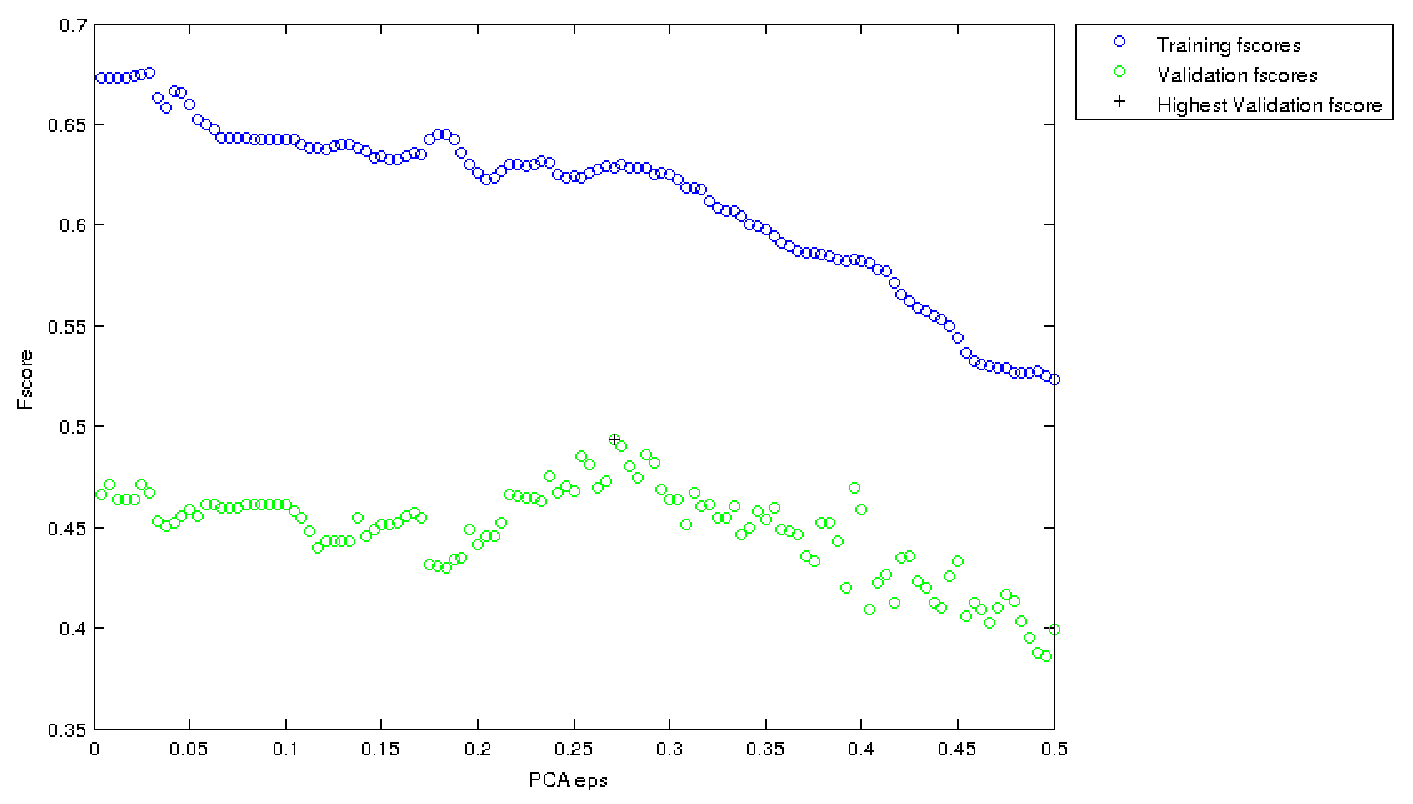
\includegraphics[scale=0.5,angle=0]{./lda_elec_range.pdf}}
	\label{fig:elecRange}
\end{center}
\end{figure}


\begin{figure}
\begin{center}
	\caption{Parties range}
	{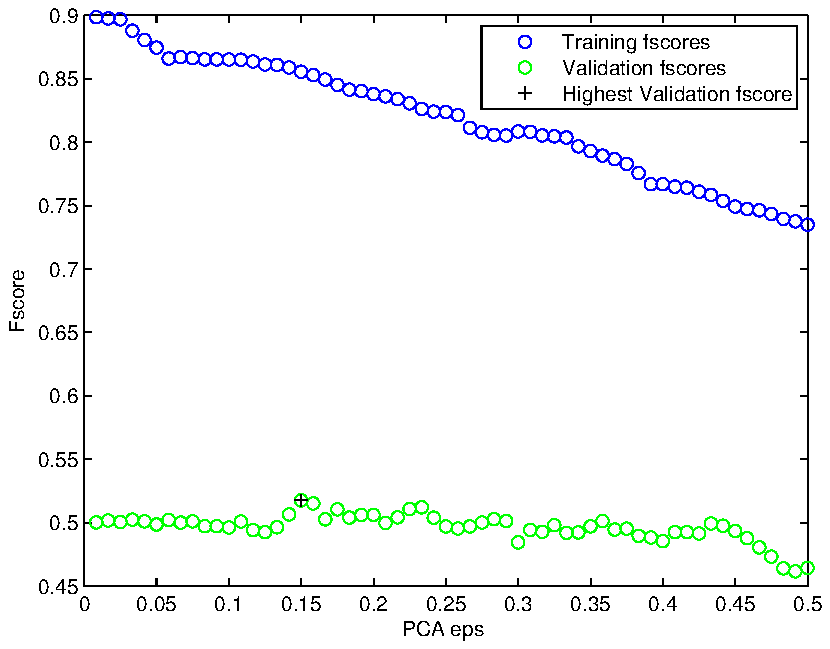
\includegraphics[scale=0.5,angle=0]{./lda_party_range.pdf}}
	\label{fig:partiesRange}
\end{center}
\end{figure}

After this we run the tests again with this delimited area and we tested the found model against the test data. Figures \ref{fig:elecTest} and \ref{fig:partiesTest} demonstrate this.

\begin{figure}
\begin{center}
	\caption{Elected estimation}
	{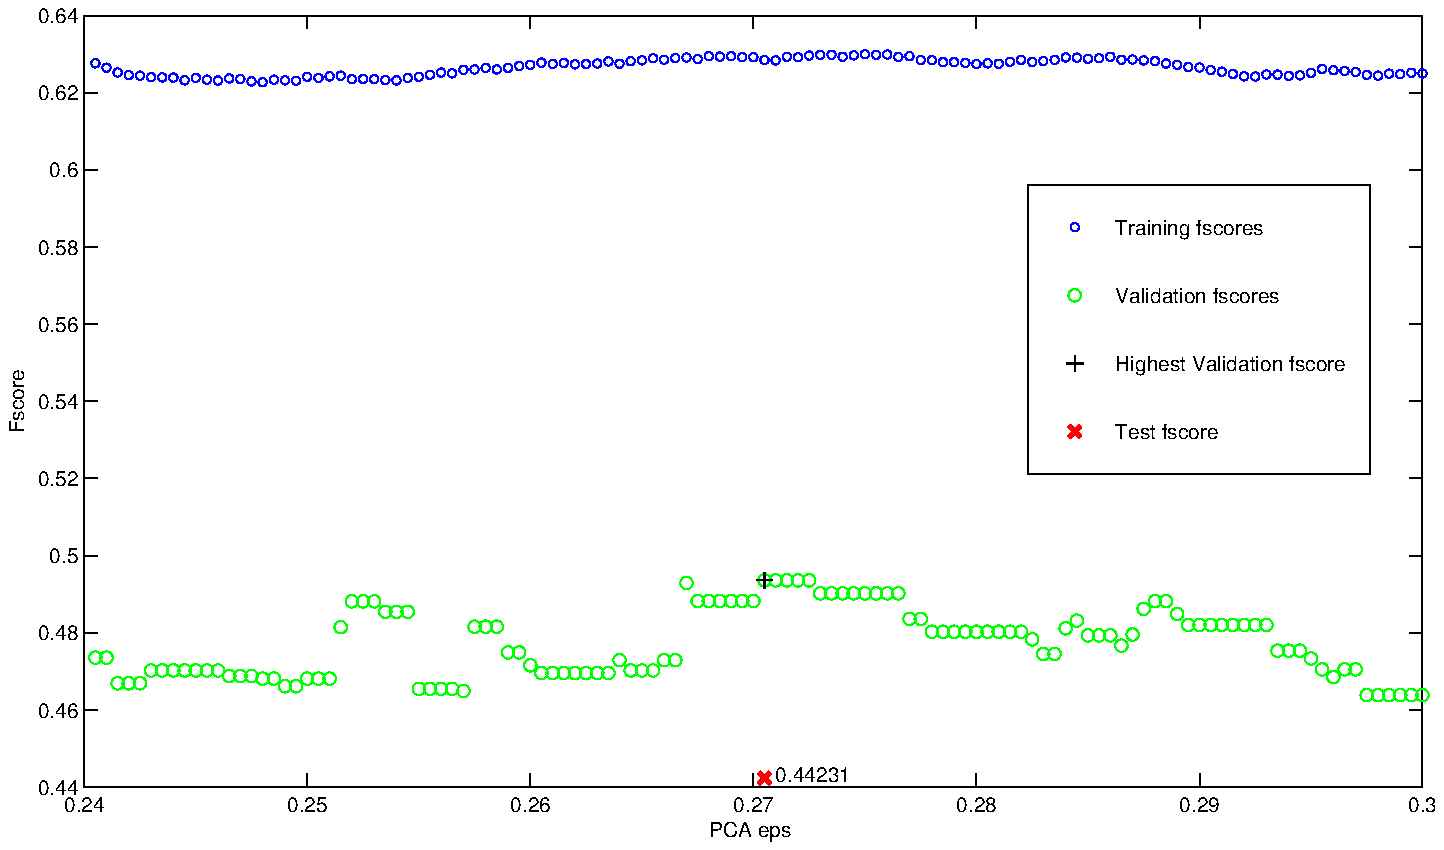
\includegraphics[scale=0.5,angle=0]{./lda_elec_test.pdf}}
	\label{fig:elecTest}
\end{center}
\end{figure}


\begin{figure}
\begin{center}
	\caption{Parties estimation}
	{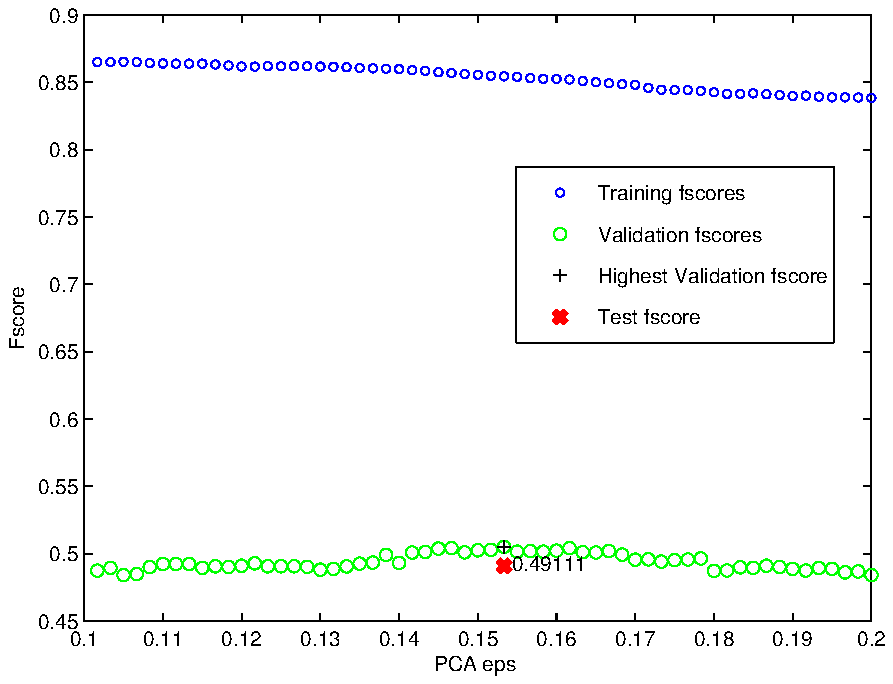
\includegraphics[scale=0.5,angle=0]{./lda_party_test.pdf}}
	\label{fig:partiesTest}
\end{center}
\end{figure}

\subsubsection{Using question groups to remove linearity}
We also tried reducing dimensionality and eliminating linear dependencies by grouping the data into distinct questions found by analysing the data. This paired with linear discriminant analysis classification yielded disappointing results: the F-score for the party data was from the lower 0.3 range and the F-score for the election data was even under 0.1.

\subsection{Bayesian methods}
\subsubsection{Naive Bayes}
PCA projections were tried from 1 to 180 principal components. The maximum score was found with projection to the 159 first PCs, giving F-score of {\bf 0.53352} with k-fold K=N/25. This was one of the best F-scores in the training set!

This projection gave F-score of 0.4829 in the test set.

\subsubsection{Tuning Gamma and Delta}
Tuning the Gamma and Delta didn’t result in much better results.

IMG PCA FROM 15:100 bayes\_gamma\_pca\_1.pdf

In PCA degrees of projection from 15 to 100 principal components the best degree was 91, with delta of 0.2637, gamma of 0.2222 and F-score 0.52453. The resulting F-score in the test set was 0.4795.

IMG PCA FROM 100:180 bayes\_gamma\_pca\_2.pdf

In PCA degrees of projection from 100 to 180 principal components the best degree was 140, with delta of 1.654113e-01, gamma of 4.444444e-01 with Matlab whining about those, and F-score 0.53491, better than the previous without tuning.

The resulting F-score in the test set was 0.4851.

It seems doubtful that PCA provides much improvement in scores, but it helps to reduce some dimensions and cut linearly dependent features which sometimes wreak havoc by causing non-positive definite covariance matrices when training models.

\section{Discussion}
\section{Reference List}
\section{Appendices}


\end{document}
